\chapter{Signed curvature}

\section{Definitions}\label{sec:def(skur)}

Suppose $\gamma$ is a smooth unit-speed plane curve,
so $\tan(s)=\gamma'(s)$ is its unit tangent vector for any $s$.

Let us rotate $\tan(s)$ by the angle $\tfrac\pi 2$ counterclockwise; 
denote the obtained vector by $\norm(s)$.
The pair $\tan(s),\norm(s)$ is an oriented orthonormal frame in the plane which is analogous to the Frenet frame
defined in Section~\ref{sec:frenet-frame};
we will keep the name \index{Frenet frame}\emph{Frenet frame} for it.

Recall that $\gamma''(s)\perp \gamma'(s)$ (see \ref{prop:a'-pertp-a''}).
Therefore 
\[\tan'(s)=\skur(s)\cdot \norm(s).\eqlbl{eq:tau'}\]\index{$\skur$}
for some real number $\skur(s)$;
the value $\skur(s)$ is called \index{signed curvature}\emph{signed curvature} of $\gamma$ at $s$.
We may use notation $\skur(s)_\gamma$ if we need to specify the curve~$\gamma$.

Note that 
\[\kur(s)=|\skur(s)|;\]
that is, up to sign, the signed curvature $\skur(s)$ equals the curvature $\kur(s)$  of $\gamma$ at $s$ defined in Section~\ref{sec:curvature};
the sign tells us in which direction it turns --- if $\gamma$ is turning left at time $s$, then $\skur (s)>0$.
If we want to emphasise that we are working with the {}\emph{nonsigned} curvature of the curve, 
we call it \index{absolute curvature}\emph{absolute curvature}.

Note that if we reverse the parametrization of $\gamma$ or change the orientation of the plane, then
the signed curvature changes its sign.

Since $\tan(s),\norm(s)$ is an orthonormal frame, we have 
\begin{align*}
\langle\tan,\tan\rangle&=1,
&
\langle\norm,\norm\rangle&=1, 
&
\langle\tan,\norm\rangle&=0,
\end{align*}
Differentiating these idenitites we get 
\begin{align*}
\langle\tan',\tan\rangle&=0,
&
\langle\norm',\norm\rangle&=0,
&
\langle\tan',\norm\rangle+\langle\tan,\norm'\rangle&=0,
\end{align*}
By \ref{eq:tau'}, $\langle\tan',\norm\rangle=\skur$ and therefore $\langle\tan,\norm'\rangle=-\skur$.
Whence we get 
\[\norm'(s)=-\skur(s)\cdot \tan(s).\eqlbl{eq:nu'}\]
The equations \ref{eq:tau'} and \ref{eq:nu'} are the Frenet formulas for plane curves. 
They can be written in matrix form as:
\[
\begin{pmatrix}
\tan'
\\
\norm'
\end{pmatrix}
=
\begin{pmatrix}
0&\skur
\\
-\skur&0
\end{pmatrix}
\cdot
\begin{pmatrix}
\tan
\\
\norm
\end{pmatrix}.
\]

\begin{thm}{Exercise}\label{ex:bike}
Let $\gamma_0\:[a,b]\to\RR^2$ be a smooth regular curve and $\tan$ its tangent indicatrix.
Consider another curve $\gamma_1\:[a,b]\to\RR^2$ defined by $\gamma_1(t)=\gamma_0(t)+\tan(t)$.
Show that
\[\length\gamma_0\le \length\gamma_1.\]

\end{thm}

The curves $\gamma_0$ and $\gamma_1$ in the exercise above describe the tracks of an idealized bicycle with  distance 1 from the rear to the front wheel.
Thus by the exercise, the front wheel must have longer track.
For more on the geometry of bicycle tracks, see the survey of Robert Foote, Mark Levi, and Serge Tabachnikov \cite{foote-levi-tabachnikov} and the references therein.

\section{Fundamental theorem of plane curves}

\begin{thm}{Theorem}\label{thm:fund-curves-2D}
Let $\skur(s)$ be a smooth real valued function defined on a real interval $\mathbb{I}$.
Then there is a smooth unit-speed curve $\gamma\:\mathbb{I}\to\RR^2$ with signed curvature $\skur(s)$.
Moreover, $\gamma$ is uniquely defined up to a rigid motion of the plane.
\end{thm}

This is the fundamental theorem of plane curves; it is a direct analog of \ref{thm:fund-curves} and it can be proved along the same lines.
We present a slightly simpler proof.
\parit{Proof.} 
Fix $s_0\in\mathbb{I}$.
Consider the function
\[\theta(s)
=
\int_{s_0}^s\skur(t)\cdot dt.\]
Note that by the fundamental theorem of calculus, we have $\theta'(s)\z=\skur(s)$ for all~$s$.

Set 
\[\tan(s)=(\cos[\theta(s)],\sin[\theta(s)])\] and let $\norm(s)$ be its counterclockwise rotation by angle $\tfrac\pi2$; so 
\[\norm(s)=(-\sin[\theta(s)],\cos[\theta(s)]).\]
Consider the curve 
\[\gamma(s)=\int_{s_0}^s\tan(s)\cdot ds.\]
Since $|\gamma'|=|\tan|=1$, the curve $\gamma$ is unit-speed and $\tan,\norm$ is its Frenet frame. 

Note that
\begin{align*}
\gamma''(s)&=\tan'(s)=
\\
&=(\cos[\theta(s)]',\sin[\theta(s)]')=
\\
&=\theta'(s)\cdot (-\sin[\theta(s)],\cos[\theta(s)])=
\\
&=\skur(s)\cdot \norm(s).
\end{align*}
So $\skur(s)$ is the signed curvature of $\gamma$ at $s$. 

This proves the existence;
it remains to prove uniqueness.

Assume $\gamma_1$ and $\gamma_2$ are two curves that satisfy the assumptions of the theorem.
Applying a rigid motion, we can assume that $\gamma_1(s_0)\z=\gamma_2(s_0)\z=0$ and the Frenet frame of both curves at $s_0$ is formed by the coordinate frame $(1,0),(0,1)$.
Let us denote by $\tan_1,\norm_1$ and $\tan_2,\norm_2$ the Frenet frames of $\gamma_1$ and $\gamma_2$ respectively.
Both triples $\gamma_i,\tan_i,\norm_i$ satisfy the following system of ordinary differential equations 
\[
\begin{cases}
\gamma_i'=\tan_i,
\\
\tan_i'=\skur\cdot\norm_i,
\\
\norm_i'=-\skur\cdot\tan_i.
\end{cases}
\]

Moreover, they have the same initial values at $s_0$.
By uniqueness of a solution of ordinary differential equation (\ref{thm:ODE}), we have $\gamma_1=\gamma_2$.
\qeds

Note that from the proof of theorem we obtain the following corollary:



\begin{thm}{Corollary}\label{cor:2D-angle}
Let $\gamma\:\mathbb{I}\to\RR^2$ be a smooth unit-speed curve and $s_0\z\in \mathbb{I}$.
Denote by $\skur$ the signed curvature of $\gamma$.
Assume an oriented $(x,y)$-coordinate system is chosen in such a way that $\gamma(s_0)$ is the origin and $\gamma'(s_0)$ points in the direction of the $x$-axis.
Then 
\[\gamma'(s)=(\cos[\theta(s)],\sin[\theta(s)]) , \]
for all $s$, where 
\[\theta(s)=\int_{s_0}^s\skur(t)\cdot dt.\]
\end{thm}


\section{Total signed curvature}

Let $\gamma\:\mathbb{I}\to\RR^2$ be a smooth unit-speed plane curve.
The \index{total signed curvature}\emph{total signed curvature} of $\gamma$, denoted by $\Psi(\gamma)$, is defined as the integral
\[\Psi(\gamma)
=
\int_\mathbb{I} \skur(s)\cdot ds,\eqlbl{eq:tsc-k}\]\index{$\Psi(\gamma)$}
where $\skur$ denotes the signed curvature of $\gamma$.

Note that if $\mathbb{I}=[a,b]$, then 
\[\Psi(\gamma)=\theta(b)-\theta(a),\eqlbl{eq:tsc-theta}\]
where $\theta$ is as in \ref{cor:2D-angle}.

If $\gamma$ is a piecewise smooth and regular plane curve, then we define its total signed curvature as the sum of the total signed curvatures of its arcs plus the sum of the \emph{signed} external angles at its joints;
it is positive if $\gamma$ turns left, negative if $\gamma$ turns right, 0 if it goes straight.
It is undefined if it turns exactly backward;
that is, if the curve has a cusp.
That is, if $\gamma$ is a concatenation of smooth and regular arcs $\gamma_1,\dots,\gamma_n$, then 
\[\Psi(\gamma)=\Psi(\gamma_1)+\dots+\Psi(\gamma_n)+\theta_1+\dots+\theta_{n-1}\]
where $\theta_i$ is the signed external angle at the joint between $\gamma_i$ and $\gamma_{i+1}$.
If $\gamma$ is closed, then the concatenation is cyclic and
\[\Psi(\gamma)=\Psi(\gamma_1)+\dots+\Psi(\gamma_n)+\theta_1+\dots+\theta_{n},\]
where $\theta_n$ is the signed external angle at the joint between $\gamma_n$ and $\gamma_1$.

Since $\left|\int \skur(s)\cdot ds\right|\le \int|\skur(s)|\cdot ds$, we have
\[|\Psi(\gamma)|\le \tc\gamma\eqlbl{eq:tsc-tc}\] 
for any smooth regular plane curve $\gamma$;
that is, the total signed curvature $\Psi$ cannot exceed the total curvature $\tc{}$ by absolute value.
Note that the equality holds if and only if the signed curvature does not change the sign.

\begin{thm}{Exercise}\label{ex:trochoids}
Trochoid is a curve traced out by a point fixed to a wheel as it rolls along a straight line.
\begin{figure}[h!]
\centering
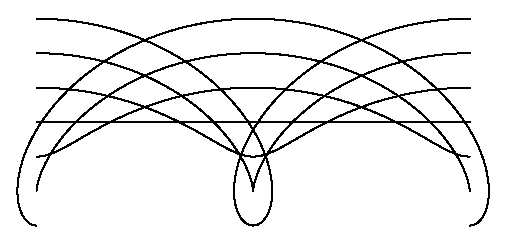
\includegraphics{asy/trochoids}
\end{figure}
A family of \index{trochoid}\emph{trochoids} $\gamma_a\:[0,2\cdot\pi]\to \RR^2$ (see the picture) can be parameterized as
\[\gamma_a(t)=(t+a\cdot \sin t, a\cdot \cos t).\]
\begin{enumerate}[(a)]
\item Given $a\in \RR$, find $\Psi(\gamma_a)$ if it is defined.
\item Given $a\in \RR$, find $\tc{\gamma_a}$.
\end{enumerate}
\end{thm}

\begin{thm}{Proposition}\label{prop:total-signed-curvature}
The total signed curvature of any closed simple smooth regular plane curve $\gamma$ is $\pm2\cdot\pi$; it is $+2\cdot\pi$
if the region bounded by $\gamma$ lies on the left from it and  $-2\cdot\pi$ otherwise.

Moreover the same statement holds for any closed piecewise simple smooth regular plane curve $\gamma$ if its total signed curvature is defined.
\end{thm}

This proposition is called sometimes \index{Umlaufsatz}\emph{Umlaufsatz}; it is a differential-geometric analog of the theorem about the sum of the internal angles of a polygon (\ref{thm:sum=(n-2)pi}) which we use in the proof.
A more conceptual proof was given by Heinz Hopf \cite{hopf1935}, \cite[p. 42]{hopf1989}.

\parit{Proof.}
Without loss of generality we may assume that $\gamma$ is oriented in such a way that the region bounded by $\gamma$ lies on the left from it.
We can also assume that it is parametrized by arc-length.

Consider a closed polygonal line $\beta=p_1\dots p_n$ inscribed in $\gamma$.
We can assume that the arcs between the vertexes are sufficiently small;
so the polygonal line is simple and each arc $\gamma_i$ from $p_i$ to $p_{i+1}$ has small total absolute curvature, say  $\tc{\gamma_i}<\pi$ for each $i$.

\begin{wrapfigure}[13]{o}{43 mm}
\vskip4mm
\centering
\includegraphics{mppics/pic-59}
\vskip4mm
\end{wrapfigure}

As usual we use indexes modulo $n$, in particular $p_{n+1}\z=p_1$.
Assume $p_i=\gamma(t_i)$.
Set 
\begin{align*}
\vec w_i&=p_{i+1}-p_i,& \vec v_i&=\gamma'(t_i),
\\
\alpha_i&=\measuredangle(\vec v_i,\vec w_i),&\beta_i&=\measuredangle(\vec w_{i-1},\vec v_i),
\end{align*}
where $\alpha_i,\beta_i\in(-\pi,\pi]$ are signed angles --- $\alpha_i$ is positive if $\vec w_i$ points to the left from $\vec v_i$.

By \ref{eq:tsc-theta}, the value
\[\Psi(\gamma_i)-\alpha_i-\beta_{i+1}\eqlbl{eq:Psi-alpha-beta}\]
is a multiple of $2\cdot\pi$.
Since $\tc{\gamma_i}<\pi$, by the chord lemma (\ref{lem:chord}), we also have that $|\alpha_i|\z+|\beta_i|<\pi$.
By \ref{eq:tsc-tc}, we have that $|\Psi(\gamma_i)|\le\tc{\gamma_i}$;
therefore the value in \ref{eq:Psi-alpha-beta} vanishes.
In other word,for each $i$ we have
\[\Psi(\gamma_i)=\alpha_i+\beta_{i+1}.\]

Note that 
\[\delta_i=\pi-\alpha_i-\beta_i\eqlbl{eq:delta=pi-alpha-beta}\] 
is the internal angle of $\beta$ at $p_i$;
$\delta_i\in (0,2\cdot\pi)$ for each $i$.
Recall that the sum of the internal angles of an $n$-gon is $(n-2)\cdot \pi$ (see \ref{thm:sum=(n-2)pi}); that is,
\[\delta_1+\dots+\delta_n=(n-2)\cdot \pi.\]
Therefore 
\[
\begin{aligned}
\Psi(\gamma)&=\Psi(\gamma_1)+\dots+\Psi(\gamma_n)=
\\
&=(\alpha_1+\beta_2)+\dots+(\alpha_n+\beta_1)=
\\
&=(\beta_1+\alpha_1)+\dots+(\beta_n+\alpha_n)=
\\
&=(\pi-\delta_1)+\dots+(\pi-\delta_n)=
\\
&=n\cdot\pi-(n-2)\cdot \pi=
\\
&=2\cdot\pi.
\end{aligned}\eqlbl{eq:delta=pi-alpha-beta-sum}\]

The case of piecewise smooth and regular curves is done the same way;
we need to subdivide the arcs in the cyclic concatenation further to meet the requirement above and instead of equation \ref{eq:delta=pi-alpha-beta} we have 
\[\delta_i=\pi-\alpha_i-\beta_i-\theta_i,\]
where $\theta_i$ is the signed external angle of $\gamma$ at $p_i$; it vanishes if the curve $\gamma$ is smooth at $p_i$.
Therefore instead of equation \ref{eq:delta=pi-alpha-beta-sum}, we have
\begin{align*}
\Psi(\gamma)&=\Psi(\gamma_1)+\dots+\Psi(\gamma_n)+\theta_1+\dots+\theta_n=
\\
&=(\alpha_1+\beta_2)+\dots+(\alpha_n+\beta_1)=
\\
&=(\beta_1+\alpha_1+\theta_1)+\dots+(\beta_n+\alpha_n+\theta_n)=
\\
&=(\pi-\delta_1)+\dots+(\pi-\delta_n)=
\\
&=n\cdot\pi-(n-2)\cdot \pi=
\\
&=2\cdot\pi.
\end{align*}
\qedsf

%???+guided exercise with hopf's proof???

\begin{thm}{Exercise}\label{ex:zero-tsc}
Draw a smooth regular closed plane curve $\gamma$ such that 

\begin{subthm}{ex:zero-tsc:0}$\Psi(\gamma)=0$;
\end{subthm}
 
\begin{subthm}{ex:zero-tsc:5}$\Psi(\gamma)=\tc\gamma=10\cdot\pi$;
\end{subthm}

\begin{subthm}{ex:zero-tsc:2-4}$\Psi(\gamma)=2\cdot \pi$ and $\tc\gamma=4\cdot\pi$.
\end{subthm}

\end{thm}

\begin{thm}{Exercise}\label{ex:length'}
Let $\gamma\:[a,b]\to\RR$ be a smooth regular plane curve with Frenet frame $\tan,\norm$.
Given a real parameter $\ell$, consider
the curve $\gamma_\ell(t)\z=\gamma(t)+\ell\cdot\norm(t)$; it is called a {}\emph{parallel curve of $\gamma$ at signed distance~$\ell$}.

\begin{subthm}{ex:length':reg}
Show that $\gamma_\ell$ is a regular curve if $\ell\cdot \skur(t)\ne 1$ for all $t$, where $\skur(t)$ denotes the signed curvature of $\gamma$.
\end{subthm}
 
\begin{subthm}{ex:length':formula}
Set $L(\ell)=\length\gamma_\ell$.
Show that 
\[L(\ell)=L(0)-\ell\cdot\Psi(\gamma)\eqlbl{eq:length(parallel-curve)}\]
for all $\ell$ sufficiently close to $0$. 
\end{subthm}

\begin{subthm}{ex:length':antiformula}
Describe an example showing that formula \ref{eq:length(parallel-curve)} does not hold for all $\ell$. 
\end{subthm}

\end{thm}


\section{Osculating circline}

\begin{thm}{Proposition}\label{prop:circline}
Given a point $p$,
a unit vector $\tan$ 
and a real number $\skur$, there is a unique smooth unit-speed curve $\sigma\:\RR\to\RR^2$ 
that starts at $p$ in the direction of $\tan$ and has constant signed curvature $\skur$.

Moreover, if $\skur=0$, then it is a line $\sigma(s)=p+s\cdot \tan$;
if $\skur\ne 0$, then $\sigma$ runs around a circle of radius $\tfrac1{|\skur|}$ with center at $p+\tfrac1\skur\cdot \norm$, where $\tan,\norm$ is an oriented orthonoral frame.
\end{thm}

Further we will use the term \index{circline}\emph{circline} for {}\emph{a circle or a line};
these are the only plane curves with constant signed curvature.

\parit{Proof.}
The proof is done by a calculation based on \ref{thm:fund-curves-2D} and \ref{cor:2D-angle}.

Suppose $s_0=0$, choose a coordinate system such that $p$ is its origin and $\tan$ points in the direction of the $x$-axis. Therefore $\norm$ points in the direction of the $y$-axis.
Then
\begin{align*}\theta(s)&=\int_{0}^s\skur\cdot dt=
\\
&=\skur\cdot s.
\end{align*}
Therefore
\[\sigma'(s)=(\cos[\skur\cdot s],\sin[\skur\cdot s]).\]
It remains to integrate the last identity.
If $\skur=0$, we get 
\[\sigma(s)=(s,0)\]
which describes the line $\sigma(s)=p+s\cdot \tan$.

If $\skur\ne 0$, we get
\[\sigma(s)=(\tfrac1\skur\cdot\sin[\skur\cdot s],
\tfrac1\skur\cdot(1-\cos[\skur\cdot s])).\]
which is the circle of radius $r=\tfrac1{|\skur|}$ centered at $(0,\tfrac1\skur)=p+\tfrac1\skur\cdot\norm$.
\qeds


\begin{wrapfigure}{r}{31 mm}
\vskip-0mm
\centering
\includegraphics{mppics/pic-21}
\vskip0mm
\end{wrapfigure}

\begin{thm}{Definition}
Let $\gamma$ be a smooth unit-speed plane curve;
denote by $\skur(s)$ the signed curvature of $\gamma$ at $s$.

The unit-speed curve $\sigma$ of constant signed curvature $\skur(s)$ that starts at $\gamma(s)$ in the direction $\gamma'(s)$ is called the \index{osculating circline}\emph{osculating circline} of $\gamma$ at~$s$.

The center and radius of the osculating circle at a given point are called \index{center of curvature}\emph{center of curvature} and \index{radius of curvature}\emph{radius of curvature} of the curve at that point.
\end{thm}

The osculating circle $\sigma_s$ can be also defined as the unique circline that has \index{order of contact}\emph{second order of contact} with $\gamma$ at $s$;
that is, $\rho(\ell)\z=o(\ell^2)$, where $\rho(\ell)$ denotes the distance from $\gamma(s+\ell)$ to $\sigma_s$.

The following exercise would is recommended to the reader familiar with the notion of \index{inversion}\emph{inversion}.

\begin{thm}{Advanced exercise}\label{ex:inverse}
Suppose $\gamma$ is a smooth regular plane curve that does not pass thru the origin.
Let $\hat \gamma$ be the inversion of $\gamma$ in the unit circle centered at the origin.
Show that osculating circline of $\hat\gamma$ at $s$ is the inversion of osculating circline of $\gamma$ at $s$.
\end{thm}

\section{Spiral lemma}
\label{spiral}

The following lemma was proved by Peter Tait \cite{tait}
and later rediscovered by Adolf Kneser \cite{kneser}.

\begin{wrapfigure}{r}{31 mm}
\vskip-4mm
\begin{lpic}[t(-0 mm),b(-2 mm),r(0 mm),l(0 mm)]{mppics/pic-61}
\end{lpic}
\end{wrapfigure}

\begin{thm}{Lemma}\label{lem:spiral}
Assume that $\gamma$ is a smooth regular plane curve with strictly decreasing positive signed curvature. Then the osculating circles of $\gamma$ are nested; that is, if $\sigma_s$ denoted the osculating circle of $\gamma$ at $s$,
then $\sigma_{s_0}$ lies in the open disc bounded by $\sigma_{s_1}$ for any $s_0<s_1$. \index{$\sigma_s$}
\end{thm}

It turns out that the osculating circles of the curve $\gamma$ give a peculiar foliation of an annulus by circles; it has the following property: if a smooth function is constant on each osculating circle it must be constant in the annulus \cite[see][Lecture 10]{fuchs-tabachnikov}.
Also note that the curve $\gamma$ is tangent to a circle of the foliation at each of its points.
However, it does not run along any of those circles.

\parit{Proof.}
Let $\tan(s),\norm(s)$ be the Frenet frame,
$\omega(s)$, $r(s)$
the center and radius of curvature of $\gamma$.
By \ref{prop:circline},
\[\omega(s)=\gamma(s)+r(s)\cdot \norm(s).\]

\begin{wrapfigure}{o}{35 mm}
\vskip-0mm
\centering
\begin{lpic}[t(-0 mm),b(-0 mm),r(0 mm),l(0 mm)]{mppics/pic-84}
\end{lpic}
\end{wrapfigure}

Since $\skur>0$, we have that $r(s)\cdot\skur(s)=1$.
Therefore applying Frenet formula \ref{eq:nu'}, we get that
\begin{align*}
\omega'(s)&=\gamma'(s)+r'(s)\cdot \norm(s)+r(s)\cdot \norm'(s)=
\\
&=\tan(s)+r'(s)\cdot \norm(s)-r(s)\cdot \skur(s)\cdot \tan(s)=
\\
&=r'(s)\cdot \norm(s).
\end{align*}
Since $\skur(s)$ is decreasing, $r(s)$ is increasing;
therefore $r'\ge 0$.
It follows that $|\omega'(s)|= r'(s)$ and $\omega'(s)$ points in the direction of $\norm(s)$.

Since $\norm'(s)=-\skur(s)\cdot\tan(s)$, the direction of $\omega'(s)$ cannot have constant direction on a nontrivial interval;
that is, the curve $s\mapsto \omega(s)$ contains no line segments.
Therefore 
\begin{align*}
|\omega(s_1)-\omega(s_0)|&<\length(\omega|_{[s_0,s_1]})=
\\
&=\int_{s_0}^{s_1}|\omega'(s)|\cdot ds=
\\
&=\int_{s_0}^{s_1}r'(s)\cdot ds=
\\
&=r(s_1)-r(s_0).
\end{align*}

In other words, the distance between the centers of $\sigma_{s_1}$ and $\sigma_{s_0}$
is strictly less than the difference between their raduses.
Therefore the osculating circle at $s_0$ lies inside the osculating circle at $s_1$ without touching it.
\qeds

{

\begin{wrapfigure}{r}{32 mm}
\vskip-4mm
\centering
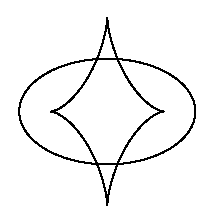
\includegraphics{asy/ellipse-astroid}
\vskip-0mm
\end{wrapfigure}

The curve $s\mapsto \omega(s)$ is called the \index{evolute}\emph{evolute} of $\gamma$; 
it traces the centers of curvature of the curve. 
The evolute of $\gamma$ can be written as 
\[\omega(t)=\gamma(t)+\tfrac1{\skur(t)}\cdot \norm(t)\] and  
in the proof we showed that $(\tfrac1{\skur})'\cdot\norm$ is its velocity vector.


\begin{thm}{Exercise}\label{ex:evolute-of-ellipse}
Show that the stretched astroid 
\[\omega(t)=(\tfrac{a^2-b^2}{a}\cdot \cos^3 t,  \tfrac{b^2-a^2}{b}\cdot\sin^3 t)\]
is an evolute of the ellipse defined by
\[\gamma(t)= (a\cdot \cos t, b\cdot\sin t).\]
\end{thm}

The following theorem states formally that 
\emph{if you drive on the plane and turn the steering wheel to the left all the time,
then you will not be able to come back to the same place.}

}

\begin{thm}{Theorem}\label{thm:spiral}
Assume $\gamma$ is a smooth regular plane curve with positive and strictly monotonic signed curvature. 
Then $\gamma$ is simple.
\end{thm}

The same statement holds true without assuming positivity of curvature; the proof requires only minor modifications.

\parit{Proof of \ref{thm:spiral}.}
Note that $\gamma(s)$ lies on the osculating circle $\sigma_s$ of $\gamma$ at $s$.
If $s_1\ne s_0$, then by lemma \ref{lem:spiral}, $\sigma_{s_0}$ does not intersect $\sigma_{s_1}$.
Therefore $\gamma(s_1)\ne \gamma(s_0)$,
hence the result.\qeds

\begin{thm}{Exercise}\label{ex:3D-spiral}
Show that a 3-dimensional analog of the theorem does not hold.
That is, there are self-intersecting smooth regular space curves with strictly monotonic curvature.
\end{thm}

\begin{thm}{Exercise}\label{ex:double-tangent}
Assume that $\gamma$ is a smooth regular plane curve with positive strictly monotonic signed curvature.

\begin{subthm}{ex:double-tangent:a}Show that no line can be tangent to $\gamma$ at two distinct points.
\end{subthm}

\begin{subthm}{ex:double-tangent:b}Show that no circle can be tangent to $\gamma$ at three distinct points. 
\end{subthm}

\end{thm} %???monotone or monotonic???

{

\begin{wrapfigure}{o}{35 mm}
\vskip-4mm
\centering
\includegraphics{mppics/pic-25}
\vskip0mm
\end{wrapfigure}

Note that part \ref{SHORT.ex:double-tangent:a} does not hold if we allow the curvature to be negative; an example is shown on the diagram.

}

\chapter{Supporting curves}

\section{Cooriented tangent curves}

Suppose $\gamma_1$ and $\gamma_2$ are smooth regular plane curves.
Recall that the curves $\gamma_1$ and $\gamma_2$ are tangent at the  time parameters $t_1$ and $t_2$
if $\gamma_1(t_1)=\gamma_2(t_2)$
and they share the tangent line at these time parameters.

In this case the point $p=\gamma_1(t_1)=\gamma_2(t_2)$ is called a \index{point of tangency}\emph{point of tangency} of the curves.
If both curves are simple, then we may say that $\gamma_1$ and $\gamma_2$ are tangent at the point $p$ 
without ambiguity.

Note that if $\gamma_1$ and $\gamma_2$ are tangent at the time parameters $t_1$ and $t_2$, 
then the velocity vectors $\gamma_1'(t_1)$ and $\gamma_2'(t_2)$ are parallel.
\begin{figure}[h!]
\vskip-0mm
\centering
\includegraphics{mppics/pic-85}
\vskip0mm
\end{figure}
If $\gamma_1'(t_1)$ and $\gamma_2'(t_2)$ point in the same direction we say that the curves are \index{cooriented!curves}\emph{cooriented},
if these directions are opposite, we say that the curves are \index{controriented!curves}\emph{controriented}.


Note that reverting the parametrization of one of the curves, cooriented curves become counteroriented and vice versa; so we can always assume that the curves are cooriented at a given point of tangency.

\section{Supporting curves}

Let $\gamma_1$ and $\gamma_2$ be two smooth regular plane curves that share a point \[p=\gamma_1(t_1)=\gamma_2(t_2)\] which is not an endpoint of any of the curves.
Suppose that there is $\eps>0$ such that the arc $\gamma_2|_{[t_2-\eps, t_2+\eps]}$ lies in a closed plane region $R$ with the arc $\gamma_1|_{[t_1-\eps, t_1+\eps]}$ in its boundary,
then we say that $\gamma_1$ \index{local support}\emph{locally supports} $\gamma_2$ at the time parameters $t_1$ and $t_2$.
If both curves are simple, then we also could say that $\gamma_1$ {}\emph{locally supports} $\gamma_2$ at the point $p$ without ambiguity.

\begin{wrapfigure}{o}{43 mm}
\vskip-3mm
\centering
\includegraphics{mppics/pic-86}
\vskip0mm
\end{wrapfigure}

If $\gamma_1$ is simple proper curve, so it divides the plane into two closed region that lie on left and right from $\gamma_1$, then we say that $\gamma_1$ \index{global support}\emph{globally supports} $\gamma_2$ at $t_2$ 
if $\gamma_2$ runs in one of these closed regions and 
$\gamma_2(t_2)$ lies on $\gamma$.

If $\gamma_2$ is a closed curve so it divides the plane into two regions a bounded inside and unbounded outside.
In this case we say if $\gamma_1$ supports $\gamma_2$ \index{support from inside}\emph{from inside} (\index{support from outside}\emph{from outside}) if $\gamma_1$ supports $\gamma_2$ and in the region inside it (respectively outside it). 

Note that if $\gamma_1$ and $\gamma_2$ share a point $p=\gamma_1(t_1)=\gamma_2(t_2)$ and not tangent at $t_1$ and $t_2$, then  $\gamma_2$ crosses $\gamma_1$ at $t_2$ moving from one of its sides to the other.
It follows that $\gamma_1$ cannot locally support $\gamma_2$ at the time parameters $t_1$ and $t_2$.
Whence we get the following:

\begin{thm}{Definition-Observation}
Let $\gamma_1$ and $\gamma_2$ be two smooth regular plane curves.
Suppose $\gamma_1$ locally supports $\gamma_2$ at time parameters $t_1$ and $t_2$.
Then $\gamma_1$ is tangent to $\gamma_2$ at $t_1$ and $t_2$.

In particular, we could say if $\gamma_1$ and $\gamma_2$ are coorineted or controriented at the time parameters $t_1$ and $t_2$.
If the curves are coorienated and the region $R$ in the definition of supporting curves lie on the right (left) from the arc of $\gamma_1$, then we say that 
$\gamma_1$ supports $\gamma_2$ from the left (respectively right).
\end{thm}

If the curves on the diagram oriented according the arrows, then $\gamma_1$ supports $\gamma_2$ from the right at $p$ (as well as $\gamma_2$ supports $\gamma_1$ from the left at $p$).

We say that a smooth regular plane curve $\gamma$ has a \index{vertex of  curve}\emph{vertex} at $s$
if the signed curvature function is critical at $s$;
that is, if $\skur'(s)_\gamma=0$.
If $\gamma$ is simple we could say that the point $p=\gamma(s)$ is a vertex of $\gamma$ without ambiguity.

\begin{thm}{Exercise}\label{ex:vertex-support}
Assume that osculating circle $\sigma_s$ of a smooth regular simple plane curve $\gamma$ locally supports $\gamma$ at $p=\gamma(s)$.
Show that $p$ is a vertex of $\gamma$.
\end{thm}

\section{Supporting test}

The following proposition resembles the second derivative test. 

\begin{thm}{Proposition}\label{prop:supporting-circline}
Let $\gamma_1$ and $\gamma_2$ be two smooth regular plane curves.

Suppose $\gamma_1$ locally supports $\gamma_2$ from the left (right) at the time parameters $t_1$ and $t_2$.
Then 
\[\skur_1(t_1)\le \skur_2(t_2)\quad(\text{respectively}\quad \skur_1(t_1)\ge \skur_2(t_2)).\]
where $\skur_1$ and $\skur_2$ denote the signed curvature of $\gamma_1$ and $\gamma_2$ respectively.

A partial converse also holds.
Namely, if $\gamma_1$ and $\gamma_2$ tangent and cooriented at the time parameters $t_1$ and $t_2$
then $\gamma_1$ locally supports $\gamma_2$ from the left (right) at the time parameters $t_1$ and $t_2$
if 
\[\skur_1(t_1)< \skur_2(t_2)\quad(\text{respectively}\quad \skur_1(t_1)> \skur_2(t_2)).\]

\end{thm}

\parit{Proof.} Without loss of generality, we can assume that $t_1=t_2=0$, the shared point $\gamma_1(0)=\gamma_2(0)$ is the origin and the velocity vectors $\gamma'_1(0)$, $\gamma'_2(0)$ point in the direction of $x$-axis.

Note that small arcs of $\gamma_1|_{[-\eps,+\eps]}$ and  $\gamma_2|_{[-\eps,+\eps]}$ can be described as a graph 
$y=f_1(x)$ and $y=f_2(x)$ for smooth functions $f_1$ and $f_2$ such that $f_i(0)=0$ and $f_i'(0)=0$.
Note that $f_1''(0)=\skur_1(0)$ and $f_2''(0)=\skur_2(0)$ (see \ref{ex:curvature-graph})

Clearly, $\gamma_1$ supports $\gamma_2$ from the left (right) if 
\[f_1(x)\le f_2(x)\quad(\text{respectively}\quad f_1(x)\ge f_2(x))\]
for all sufficiently small values $x$.
Applying the second derivative test, we get the result.
\qeds


\begin{thm}{Advanced exercise}\label{ex:support}
Let $\gamma_0$ and $\gamma_1$ be two smooth unit-speed simple plane curves that are tangent and cooriented at the point $p\z=\gamma_0(0)=\gamma_1(0)$.
Assume $\skur_0(s)\le\skur_1(s)$ for any $s$.
Show that $\gamma_0$ locally supports $\gamma_1$ from the right at $p$.

Give an example of two proper curves $\gamma_0$ and $\gamma_1$ satisfying the above condition such that $\gamma_0$ does not globally support $\gamma_1$ at $p$.
\end{thm}

Note that according to \ref{thm:DNA} for any closed smooth regular curve that runs in a unit disc, the average of its absolute curvature at least 1; in particular it has a point with absolute curvature at lest 1.
The following exercise says that the last statement holds for loops.

\begin{thm}{Exercise}\label{ex:in-circle}
Assume a closed smooth regular plane loop $\gamma$ runs in a unit disc.
Show that there is a point on $\gamma$ with absolute curvature at least 1.
\end{thm}


\begin{thm}{Exercise}\label{ex:between-parallels-1}
Assume a closed smooth regular plane curve $\gamma$ runs between parallel lines on distance 2 from each other.
Show that there is a point on $\gamma$ with absolute curvature at least 1.

Try to prove the same for a smooth regular plane loop.
\end{thm}

\begin{thm}{Exercise}\label{ex:in-triangle}
Assume a closed smooth regular plane curve $\gamma$ runs inside of a triangle $\triangle$ with inradius 1; that is, the inscribed circle of $\triangle$ has radius 1.
Show that there is a point on $\gamma$ with absolute curvature at least~$1$.
\end{thm}

The exercise above is a baby case of a \ref{ex:moon-rad}.

{

\begin{wrapfigure}{o}{35 mm}
\vskip-4mm
\centering
\includegraphics{mppics/pic-70}
\vskip0mm
\end{wrapfigure}

\begin{thm}{Exercise}\label{ex:lens}
Let $F$ be a plane figure bounded by two circle arcs $\sigma_1$ and $\sigma_2$ of signed curvature 1 that run from $x$ to $y$.
Suppose $\sigma_1$ is a shorter than $\sigma_2$.
Assume a simple arc $\gamma$ runs in $F$ and has the end points on $\sigma_1$.
Show that the absolute curvature of $\gamma$ is at least 1 at some parameter value.

\end{thm}

}

\section{Convex curves}

Recall that a plane curve is convex if it bounds a convex region.

\begin{thm}{Proposition}\label{prop:convex}
Suppose that a closed simple plane curve $\gamma$ bounds a figure $F$.
Then $F$ is convex if and only if the signed curvature of $\gamma$ does not change sign.
\end{thm}


\begin{thm}{Lens lemma}\label{lem:lens}
Let $\gamma$ be a smooth regular simple plane curve that runs from $x$ to $y$.
Assume that $\gamma$ runs on the right side (left side) of the oriented line $xy$ and only its endpoints $x$ and $y$ lie on the line.
Then $\gamma$ has a point with positive (respectively negative) signed curvature.
\end{thm}

{

\begin{wrapfigure}{r}{35 mm}
\vskip-6mm
\centering
\includegraphics{mppics/pic-22}
\vskip0mm
\end{wrapfigure}

Note that the lemma fails for curves with self-intersections;
the curve $\gamma$ on the diagram always turns right, 
so it has negative curvature everywhere, but it lies on the right side of the line $xy$.

}

\parit{Proof.}
Choose points $p$ and $q$ on the line $xy$
so that the points $p, x, y, q$ appear in that order.
We can assume that $p$ and $q$ lie sufficiently far from $x$ and $y$, so that the half-disc with diameter $pq$ contains $\gamma$.

Consider the smallest disc segment with chord $[pq]$ that contains $\gamma$.
Note that its arc $\sigma$ supports $\gamma$ at some point $w=\gamma(t_0)$.

\begin{wrapfigure}{l}{50 mm}
\centering
\includegraphics{mppics/pic-24}
\bigskip
\includegraphics{mppics/pic-23}
\end{wrapfigure}

Let us parameterise $\sigma$ from $p$ to $q$.
Note that the $\gamma$ and $\sigma$ are tangent and cooriented at $w$.
If not, then the arc of $\gamma$ from $w$ to $y$ would be trapped in the curvelinear triangle $xwp$ bounded by arcs of $\sigma$, $\gamma$ and the line segment $[px]$.
But this is impossible since $y$ does not belong to this triangle.

It follows that $\sigma$ supports $\gamma$ at $t_0$ from the right.
By \ref{prop:supporting-circline}, 
\[\skur(t_0)_\gamma\ge \skur_\sigma >0.\]
\qedsf

\begin{wrapfigure}{o}{50 mm}
\vskip-6mm
\centering
\includegraphics{mppics/pic-230}
\vskip0mm
\end{wrapfigure}

\parit{Remark.}
Instead of taking the minimal disc segment, one can take a point $w$ on $\gamma$ that maximizes the distance to the line $xy$.
The same argument shows that the curvature at $w$ is nonnegative, which is slightly weaker than the required positive curvature.

\begin{wrapfigure}{o}{35 mm}
\centering
\includegraphics{mppics/pic-68}
\vskip0mm
\end{wrapfigure}

\parit{Proof of \ref{prop:convex}.}
If $F$ is convex, then every tangent line of $\gamma$ supports $\gamma$.
If a point moves along $\gamma$, the figure $F$ has to stay on one side from its tangent line;
that is, we can assume that each tangent line supports $\gamma$ on one side, say on the right.
Since line has vanishing curvature, the supporting test (\ref{prop:supporting-circline}) implies that $\skur\ge 0$ at each point.

Denote by $K$ the convex hull of $F$.
If $F$ is not convex, then $F$ is a proper subset of $K$.
Therefore $\partial K$ contains a line segment that is not a part of $\partial F$.
In other words, there is a line that supports $\gamma$ at two points, say $x$ and $y$ that divide $\gamma$ in two arcs $\gamma_1$ and $\gamma_2$, both distinct from the line segment $[x,y]$.

Note the one of the arcs $\gamma_1$ or $\gamma_2$ is parametrized from $x$ to $y$ and the other from $y$ to $x$.
Passing to a smaller arc if necessary we can ensure that only its endpoints lie on the line. 
Applying the lens lemma, we get that the arcs $\gamma_1$ and $\gamma_2$ contain points with curvatures of opposite signs.

That is, if $F$ is not convex, then curvature of $\gamma$ changes sign.
Equivalently: if curvature of $\gamma$ does not change sign, then $F$ is convex.
\qeds

\begin{thm}{Exercise}\label{ex:convex small}
Suppose $\gamma$ is a smooth regular simple closed convex plane curve of diameter larger than 2.
Show that $\gamma$ has a point with absolute curvature less than 1.
\end{thm}

\begin{thm}{Exercise}\label{ex:line-curve-intersections}
Suppose $\gamma$ is a simple smooth regular curve in the plane with positive curvature.
Assume $\gamma$ crosses a line $\ell$ at the points $p_1,p_2,\dots p_n$ and these points appear on $\gamma$ in the same order.

\begin{subthm}{ex:line-curve-intersections:a} Show that $p_2$ cannot lie between $p_1$ and $p_3$ on $\ell$.
\end{subthm}

\begin{subthm}{ex:line-curve-intersections:b} Show that if $p_3$ lies between $p_1$ and $p_2$ on $\ell$, then the points appear on $\ell$ in the following order:  
\[p_1,p_3,\dots,p_4 ,p_2.\]

\end{subthm}

\begin{subthm}{ex:line-curve-intersections:c}
Describe all possible orders of $p_i$ on $\ell$.

\end{subthm}

\end{thm}

\section{Moon in a puddle}

The following theorem is a slight generalization of the theorem proved by Vladimir Ionin and German Pestov in \cite{ionin-pestov}.
For convex curves, this result was known earlier \cite[\S 24]{blaschke}.


\begin{wrapfigure}{r}{12 mm}
\vskip-0mm
\centering
\includegraphics{mppics/pic-67}
\vskip0mm
\end{wrapfigure}

\begin{thm}{Theorem}\label{thm:moon-orginal}
Assume $\gamma$ is a simple closed smooth regular plane loop with absolute curvature bounded by 1.
Then it surrounds a unit disc.
\end{thm}

This theorem gives a simple but nontrivial example of the so-called \index{local to global theorem}\emph{local to global theorems} --- based on some local data (in this case the curvature of a curve) we conclude a global property (in this case existence of a large disc surrounded by the curve).

{

\begin{wrapfigure}{r}{32 mm}
\vskip-4mm
\centering
\includegraphics{mppics/pic-62}
\vskip0mm
\end{wrapfigure}

A straightforward approach would be to start with some disc in the region bounded by the curve and blow it up to maximize its radius.
However, as one may see from the diagram it does not always lead to a solution --- a closed plane curve of curvature at most 1 may surround a disc of radius smaller than 1 that cannot be enlarged continuously.

}

\begin{thm}{Key lemma}\label{thm:moon}
Assume $\gamma$ is a simple closed smooth regular plane loop.
Then at one point of $\gamma$ (distinct from its base) its osculating circle $\sigma$ globally support $\gamma$ from the inside.
\end{thm}

First let us show that the theorem follows from the lemma.

\parit{Proof of \ref{thm:moon-orginal} modulo \ref{thm:moon}.}
Since $\gamma$ has absolute curvature at most 1, each osculating circle has radius at least 1.
According to the key lemma one of the osculating circles $\sigma$ globally support $\gamma$ from inside.
In particular $\sigma$ lies inside of $\gamma$, whence the result.
\qeds

\parit{Proof of \ref{thm:moon}.}
Denote by $F$ the closed region surrounded by $\gamma$.
We need to show that one osculating circle lies completely in $F$.
Assume contrary; that is, the osculating circle at each point $p\in \gamma$ does not lie in $F$.

\begin{figure}[h!]%{r}{38 mm}
\vskip-0mm
\centering
\includegraphics{mppics/pic-32}
\vskip0mm
\end{figure}

Given a point $p\in\gamma$ let us consider the maximal circle $\sigma$ that lies completely in $F$ and tangent to $\gamma$ at $p$.
Note that $\sigma$ has to touch $\gamma$ at another point;
otherwise if we increase its radius $r$ slightly the resulting circle will still stay in $F$.
The circle $\sigma$ will be called the {}\emph{incircle} of $F$ at $p$.


Fix a point $p_1$ and let $\sigma_1$ be the incircle at $p_1$.
Denote by $\gamma_1$ an arc of $\gamma$ from $p_1$ to a first point $q_1$ on $\sigma_1$.
Denote by $\hat\sigma_1$ and $\check\sigma_1$ two arcs of $\sigma_1$ from $p_1$ to $q_1$ such that the cyclic concatenation of $\hat\sigma_1$ and $\gamma_1$ surrounds $\check\sigma_1$. 

{

\begin{wrapfigure}{o}{32 mm}
\vskip-4mm
\centering
\includegraphics{mppics/pic-64}
\caption*{The ovals pretend to be circles.}
\vskip0mm
\end{wrapfigure}

Let $p_2$ be the midpoint of $\gamma_1$ and $\sigma_2$ be the incircle at $p_2$.

Note that $\sigma_2$ cannot intersect $\hat\sigma_1$.
Otherwise, if $\sigma_2$ intersects $\hat\sigma_1$ at some point $s$, then $\sigma_2$ has to have two more common points with $\check\sigma_1$, say $x$ and $y$ --- one for each arc of $\sigma_2$ from $p_2$ to $s$.
Therefore $\sigma_1\z=\sigma_2$ as two circles with three common points: $s$, $x$, and $y$. 
On the other hand, by construction, we have that $p_2\in \sigma_2$ and $p_2\notin \sigma_1$ --- a contradiction.


}

Recall that $\sigma_2$ has to touch $\gamma$ at another point.
From above it follows that it can only touch $\gamma_1$ and therefore we can choose an arc $\gamma_2\subset \gamma_1$ that runs from $p_2$ to a first point $q_2$ on $\sigma_2$.
Note that by construction we have that
\[\length \gamma_2< \tfrac12\cdot\length\gamma_1.\eqlbl{eq:length<length/2}\]

Repeating this construction recursively,
we get an infinite sequence of arcs $\gamma_1\supset \gamma_2\supset\dots$;
by \ref{eq:length<length/2}, we also get that 
\[\length\gamma_n\to0\quad\text{as}\quad n\to\infty.\] 
Therefore the intersection 
\[\bigcap_n\gamma_n\]
contains a single point; denote it by $p_\infty$.

Let $\sigma_\infty$ be the incircle at $p_\infty$; it has to touch $\gamma$ at another point, say $q_\infty$.
The same argument as above shows that $q_\infty\in\gamma_n$ for any $n$.
It follows that $q_\infty =p_\infty$ --- a contradiction.
\qeds

\begin{thm}{Exercise}\label{ex:moon-rad}
Assume that a closed smooth regular curve $\gamma$ lies in a figure $F$ bounded by a closed simple plane curve.
Suppose that $R$ is the maximal radius of discs that lies in $F$.
Show that absolute curvature of $\gamma$ is at least $\tfrac1R$ at some parameter value.
\end{thm}


\section{Four-vertex theorem}

{

\begin{wrapfigure}{o}{20 mm}
\vskip-4mm
\centering
\includegraphics{mppics/pic-26}
\vskip0mm
\end{wrapfigure}

Recall that a vertex of a smooth regular curve is defined as a critical point of its signed curvature;
in particular, any local minimum (or maximum) of the signed curvature is a vertex.
For example, every point of a circle is its vertex.

\begin{thm}{Four-vertex theorem}\label{thm:4-vert}
Any smooth regular simple plane curve has at least four
vertices.
\end{thm}

}

Evidently any closed smooth regular curve has at least two vertexes --- where the minimum and the maximum of the curvature are attained.
On the diagram the vertexes are marked;
the first curve has one self-intersection and exactly two vertexes;
the second curve has exactly four vertexes and no self-intersections.

The four-vertex theorem was first proved by Syamadas Mukhopadhyaya \cite{mukhopadhyaya} for convex curves.
It has a number of different proofs and generalizations.
One of my favorite proofs was given by Robert Osserman \cite{osserman}.
We give another proof based on the key lemma in the previous section.
It proves the following stronger statement.

\begin{thm}{Theorem}\label{thm:4-vert-supporting}
Any smooth regular simple plane curve has is globally supported by its osculating circle at least at 4 distinct points; two from inside and two from outside.
\end{thm}

{

\begin{wrapfigure}{o}{33 mm}
\vskip-2mm
\centering
\includegraphics{mppics/pic-63}
\vskip0mm
\end{wrapfigure}

\parit{Proof of \ref{thm:4-vert} modulo \ref{thm:4-vert-supporting}.}
First note that if an osculating circline $\sigma$ at a point $p$ supports $\gamma$ locally, then $p$ is a vertex.
Indeed, if $p$ is not a vertex, then a small arc around $p$ has monotonic curvature.
Applying the spiral lemma (\ref{lem:spiral}) we get that the osculating circles at this arc are nested.
In particular the curve $\gamma$ crosses $\sigma$ at $p$ and therefore $\sigma$ is does not locally support $\gamma$ at $p$.
\qeds

}

\parit{Proof of \ref{thm:4-vert-supporting}.}
According to key lemma (\ref{thm:moon}), there is a point $p\in\gamma$ such that its osculating circle supports $\gamma$ from inside.
The curve $\gamma$ can be considered as a loop with the base at $p$.
Therefore the key lemma implies existence of another point $q\in\gamma$ with the same property.

It shows the existence of two osculating circles that support $\gamma$ from inside;
it remains to show existence of two osculating circles that support $\gamma$ from outside.

In order to get the osculating circles supporting $\gamma$ from outside, one can repeat the proof of key lemma taking instead of incircle the circline of maximal signed curvature that supports the curve from outside, assuming that $\gamma$ is oriented so that the region on the left from it is bounded.%

(Alternatively, if one applies to $\gamma$ an inverse with the center inside $\gamma$, then the obtained curve $\gamma_1$ also has  two osculating circles that support $\gamma_1$ from inside.
According to \ref{ex:inverse}, these osculating circlines are inverses of the circlines osculating to $\gamma$.
Note that the rigion lying inside of $\gamma$ is mapped to the region outside of $\gamma_1$ and the other way around.
Therefore these two circlines correspond to the osculating circlines supporting $\gamma$ from outside.)
\qeds

\begin{wrapfigure}[5]{r}{25 mm}
\vskip-7mm
\centering
\includegraphics{mppics/pic-65}
\vskip0mm
\end{wrapfigure}

\begin{thm}{Advanced exercise}\label{ex:curve-crosses-circle}
Suppose $\gamma$ is a closed simple smooth regular plane curve and $\sigma$ is a circle.
Assume $\gamma$ crosses $\sigma$ at the points $p_1,\dots,p_{2{\cdot} n}$ and these points appear in the same cycle order on $\gamma$ and on $\sigma$.
Show that $\gamma$ has at least $2\cdot n$ vertexes.

Construct an example of a closed simple smooth regular plane curve $\gamma$ with only 4 vertexes that crosses a given circle at arbitrarily many points. 
\end{thm}

